\chapter*{How to \sectionsovs}

Any lunatic can do some martial arts classes, go for a couple of rounds of Cuban Salsa and come up with the idea to combine the two (the mere existence of this manifest sort of proves this point), but the secret sauce (pun intended) is in describing \textit{how} to combine the two, which is exactly what will be done in this chapter. \\
The purpose is not to do a complete enumeration of all possible combinations of Cuban Salsa figures with attacks and defences from all sub-categories of martial arts, but to demonstrate \textit{some} ways in which to combine the two, that will allow the reader to get started with experimenting on the dance floor and take part in the cancerous/viral growth of the \sovs underworld.\\
If you are totally new to either Cuban Salsa or the martial arts, you may very well benefit from pausing the consumption of this manifest, do an internet search for ``Cuban Salsa intro course'' or ``basic punching'' respectively and invest a total of 15 minutes in whatever online videos will undoubtedly be presented in abbundance. The popular online video services have brief demonstrations of all salsa figures listed here, and a 40 second demonstration will probably do more for the overall understanding of a figure, than what my limited skills in terms of drawing and providing textual descriptions can. \\

\subsection*{Rules \& ground principles of \sovs}
On the dance floor, \sovs imposes the following few and easy-to-remember rules and restrictions:

\begin{enumerate}
  \item as in Cuban Salsa, the \dude is responsible for \textit{leading}
  \item only the \gal is allowed to attack
  \item any attack and defence is allowed, as long as it does not obstruct the continuation of the dance
\end{enumerate}

The rule oulined in 3), is formalized by the \text{The Flow Must Go On}-definition:

\begin{definition}[The Flow Must Go On]
\gal is allowed to attack \dude in any and all ways thinkable, that would not prevent the succesful execution of a \textit{Rueda de Casino} given proper defence by \dude
\end{definition}

Another way of saying this is: \textit{``do what you must, but make sure to be done by the end of the figure''}. Yet another way to say the same thing is: \textit{``you may kill your partner, but don't kill the \textbf{rhythm}!''}.\\
In the descriptions that follow, parts of the currently established \sovs glossary is used. The complete \sovs nomenclature as of the current time of writing, is presented in the following chapter. 

\pagebreak{}
\section*{Examples of figures}
\subsection*{\Sovsguapea [\Salsaguapea]}
\begin{center}
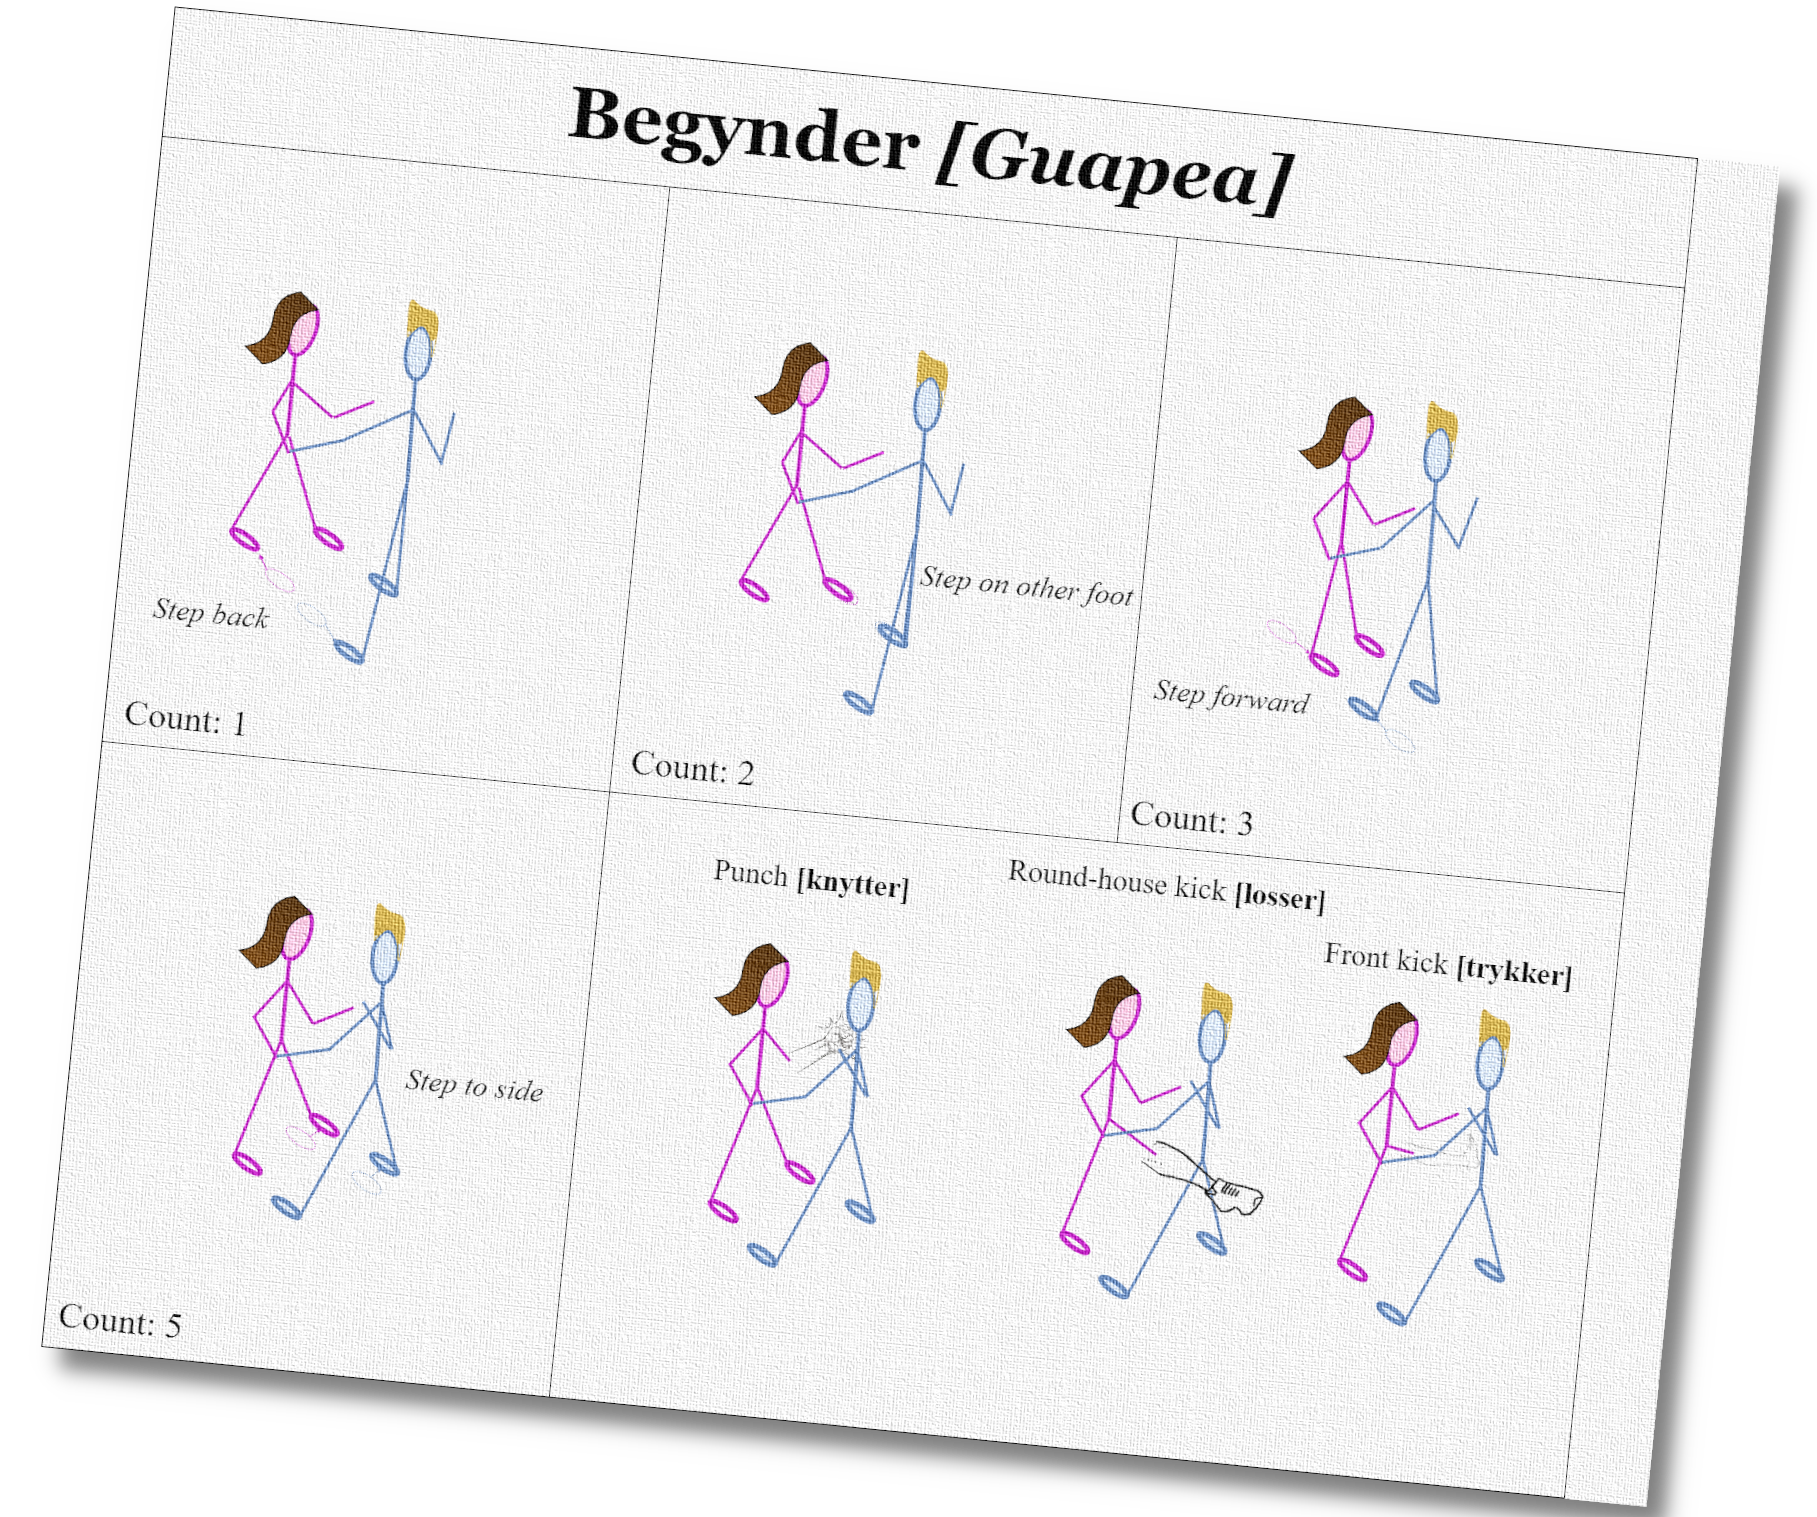
\includegraphics[scale=0.15]{02-Description/diagram-guapea-present}
\end{center}


\subparagraph*{Description}
If you, filled to the brim with anticipation of becoming the next Latin Dance God take your first Cuban Salsa intro class, it is very likely that you will first be shown a few basic steps, and when it comes time to partner up, the \salsaguapea is the first series of steps that you are taught. In \sovs, we call this same move \sovsguapea. And why is that you ask? Because it is so darn \textit{easy}!\\
\Sovsguapea starts off in the open position, with the 2 facing each other and \dude holding \scactorf{Gal's} \textbf{right} hand in his own \textbf{left} hand. On the first count both of them step back on the foot closest to the hand used for holding hands (i.e. \dude steps back on his left foot and \gal steps back on her right foot). On the second count, both step in place with the opposite foot and on the third count they both bring their hind foot forward to it's starting position. In salsa, counts 4 and 8 are generally upheld like the Abrahamic religions uphold their day of rest, and as such, are spent on quiet contemplation. On count 5, both parties step outwards with the foot closest to their \textit{free} hand as their free hands meet in the middle, palms facing towards each other. On count 6, both step in place with their opposite foot, and on count 7 they return to the starting position. 
\subparagraph*{Suggestions for attacking}
The most obvious times for \gal to attack is when she is already engaged in forward movement, either as she steps forward on count 3, or as she brings her hand towards \dude on count 5.\\
Seeing as the distance between the 2 is rather narrow, it can be hard for her to land a \atttrykker (forward-pushing kick), but the distance is quite suitable for a \attlosser (round-house kick) and pretty much any type of punch should be well within reach of it's target. If \gal is feeling frisky, she might even go for a little combination punching and try to hit \dude with for instance a quick \textit{jab-hook combo} or a \attflemming (faking a punch to the head, and diving for a weaselly gut-punch). Really, the sky is the limit!  


\pagebreak{}
\section*{\Sovsdile [\Salsadile]}
\begin{center}
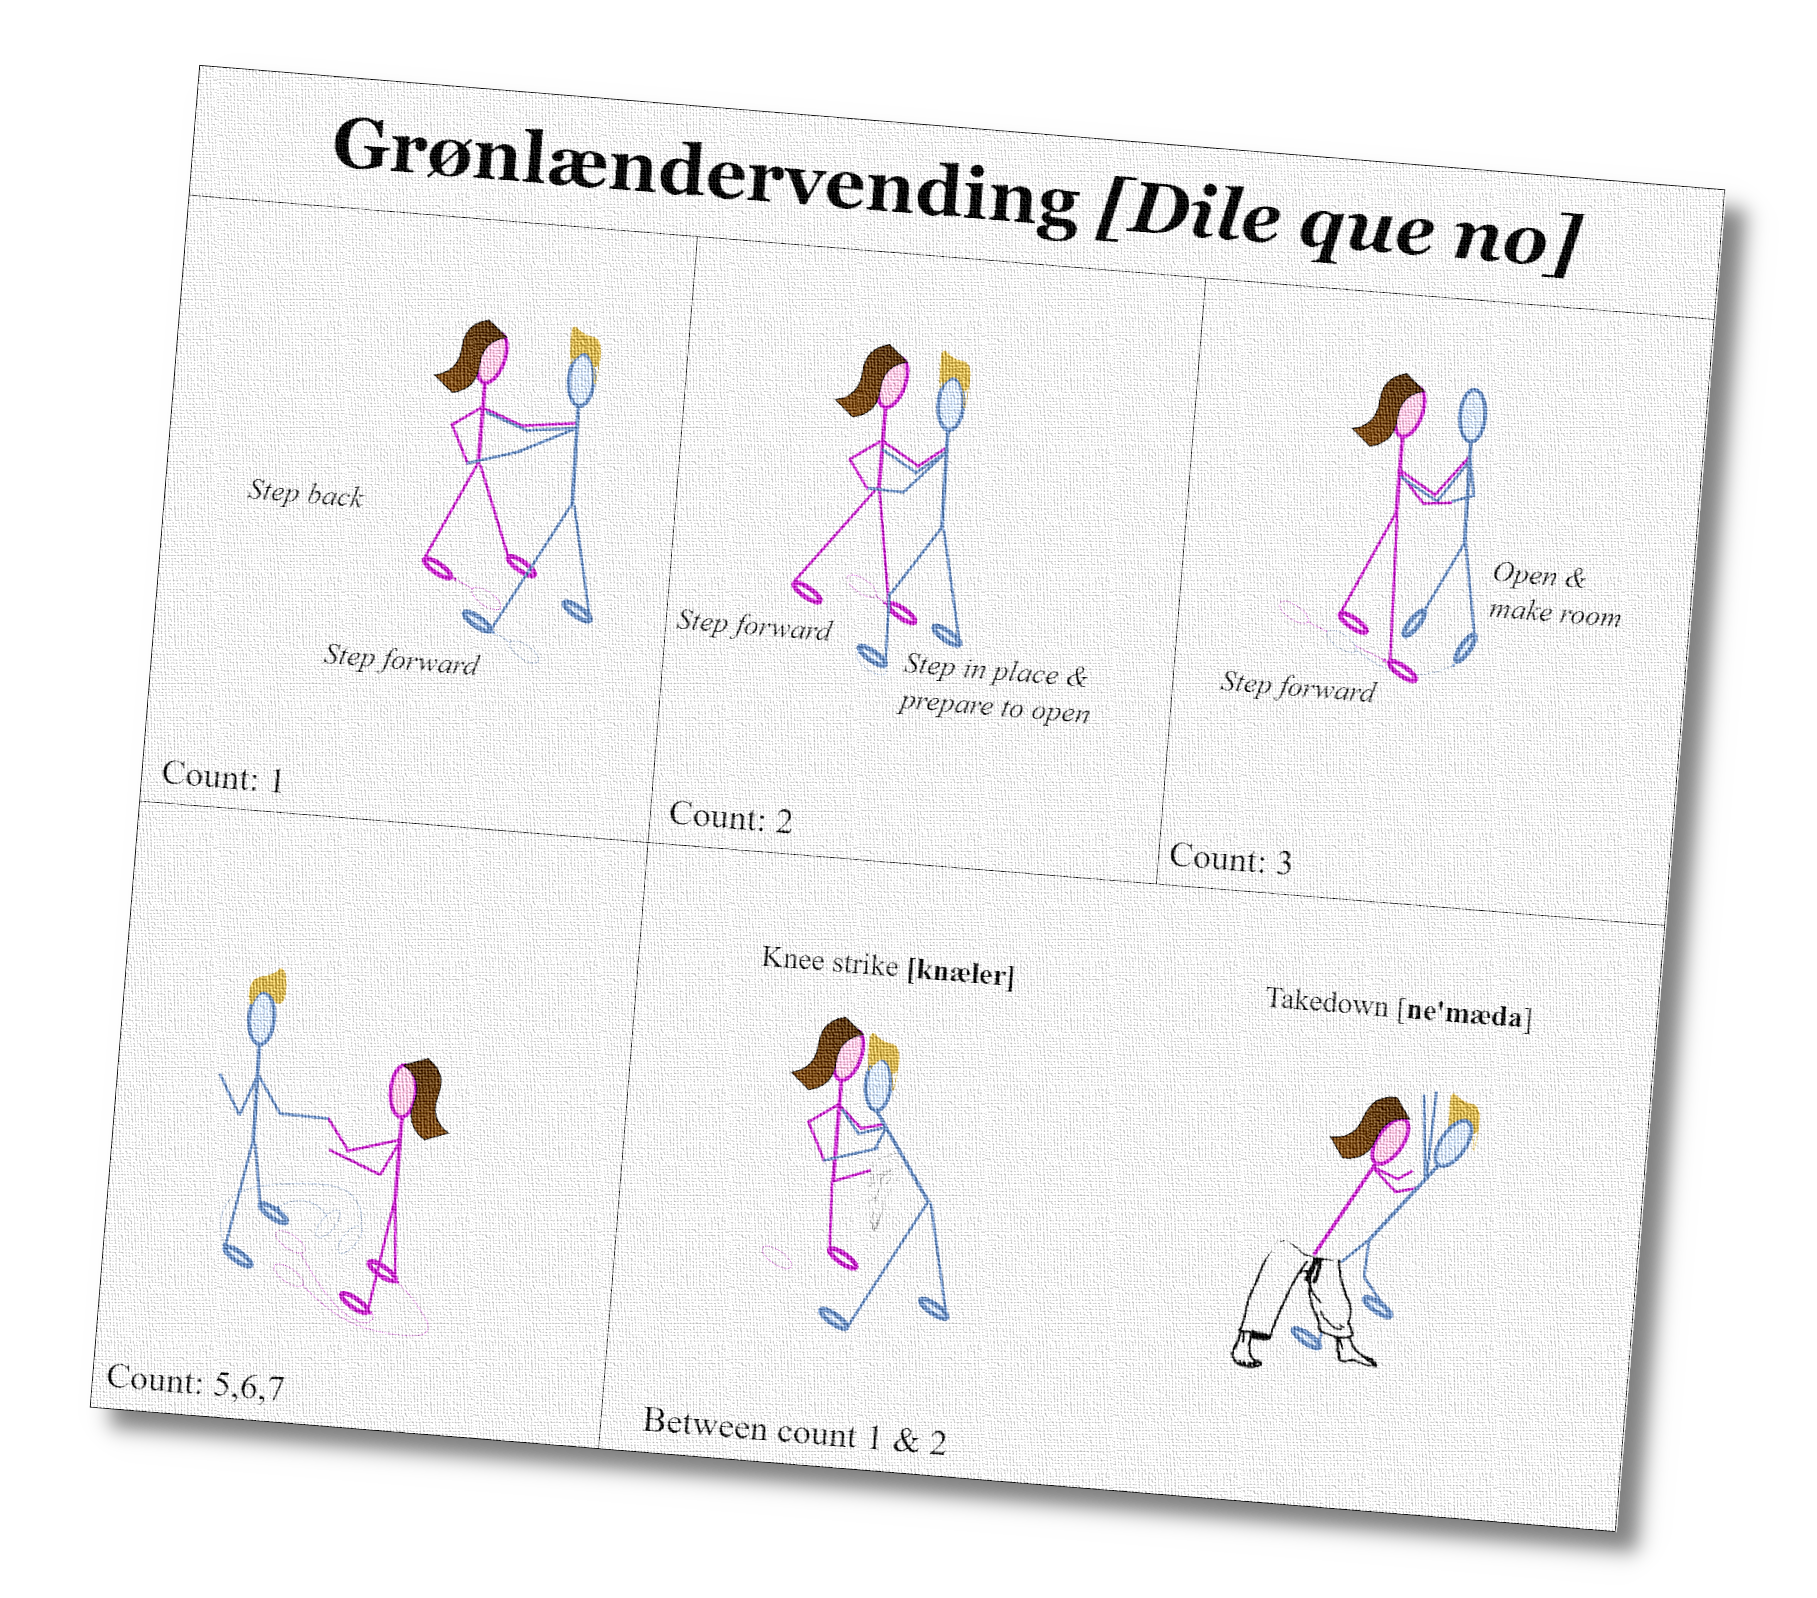
\includegraphics[scale=0.15]{02-Description/diagram-dile-que-no-present}
\end{center}
\subparagraph*{Description}
\Salsadile is in Cuban Salsa used extensively as a part in many other figures, often as the finishing move that brings the two parties back to their starting position, as they change place and direction through the 8 counts. \\
The move is initiated by \dude as he steps towards \gal with his \textbf{left} foot on count 1 and she takes a step back on her \textbf{right} foot. If \dude considers himself a proper gentleman, he will let \gal know what is coming by applying a little more push forward than usual with his left hand. On count 2, \dude takes a small step in-place with his right foot, and prepares to pivot his body leftwards around the axis of his right foot, and \gal takes a small step forward with her left foot. On count 3, \dude completes his pivot and thereby opens an alley for \gal to walk in, as she steps forward with her right foot. \\
Count 5,6 and 7 is pretty much all about the two coming into alignment with each other, both of them now facing the opposite direction of what they did at the start of the move. 
\subparagraph*{Suggestions for attacking}
The  aggresive consumption of territory on count 1 by \dude , opens for some interesting ways for \gal to establish boundaries. If \dude is showing improper balance and is leaning too much forward as he approaches, it is a perfect time for a little impact-testing of his ribcage or abdomen with a powerful \attkneeler (knee strike). Staying in the clinch/BDSM parts of the martial arts, she also has a perfect opportunity to land either a \attrambuk (horizontal elbow strike) or a \attsuperman (diagonally downward cutting elbow), and if on the other hand she really wants to show her interest in him (or she is just more of a \textit{ground n' pound}-style fighter), she could go for the \atttakedown and finish off in mount. 

\pagebreak{}
\section*{\Sovsvuelta [\Salsavuelta]}
\begin{center}
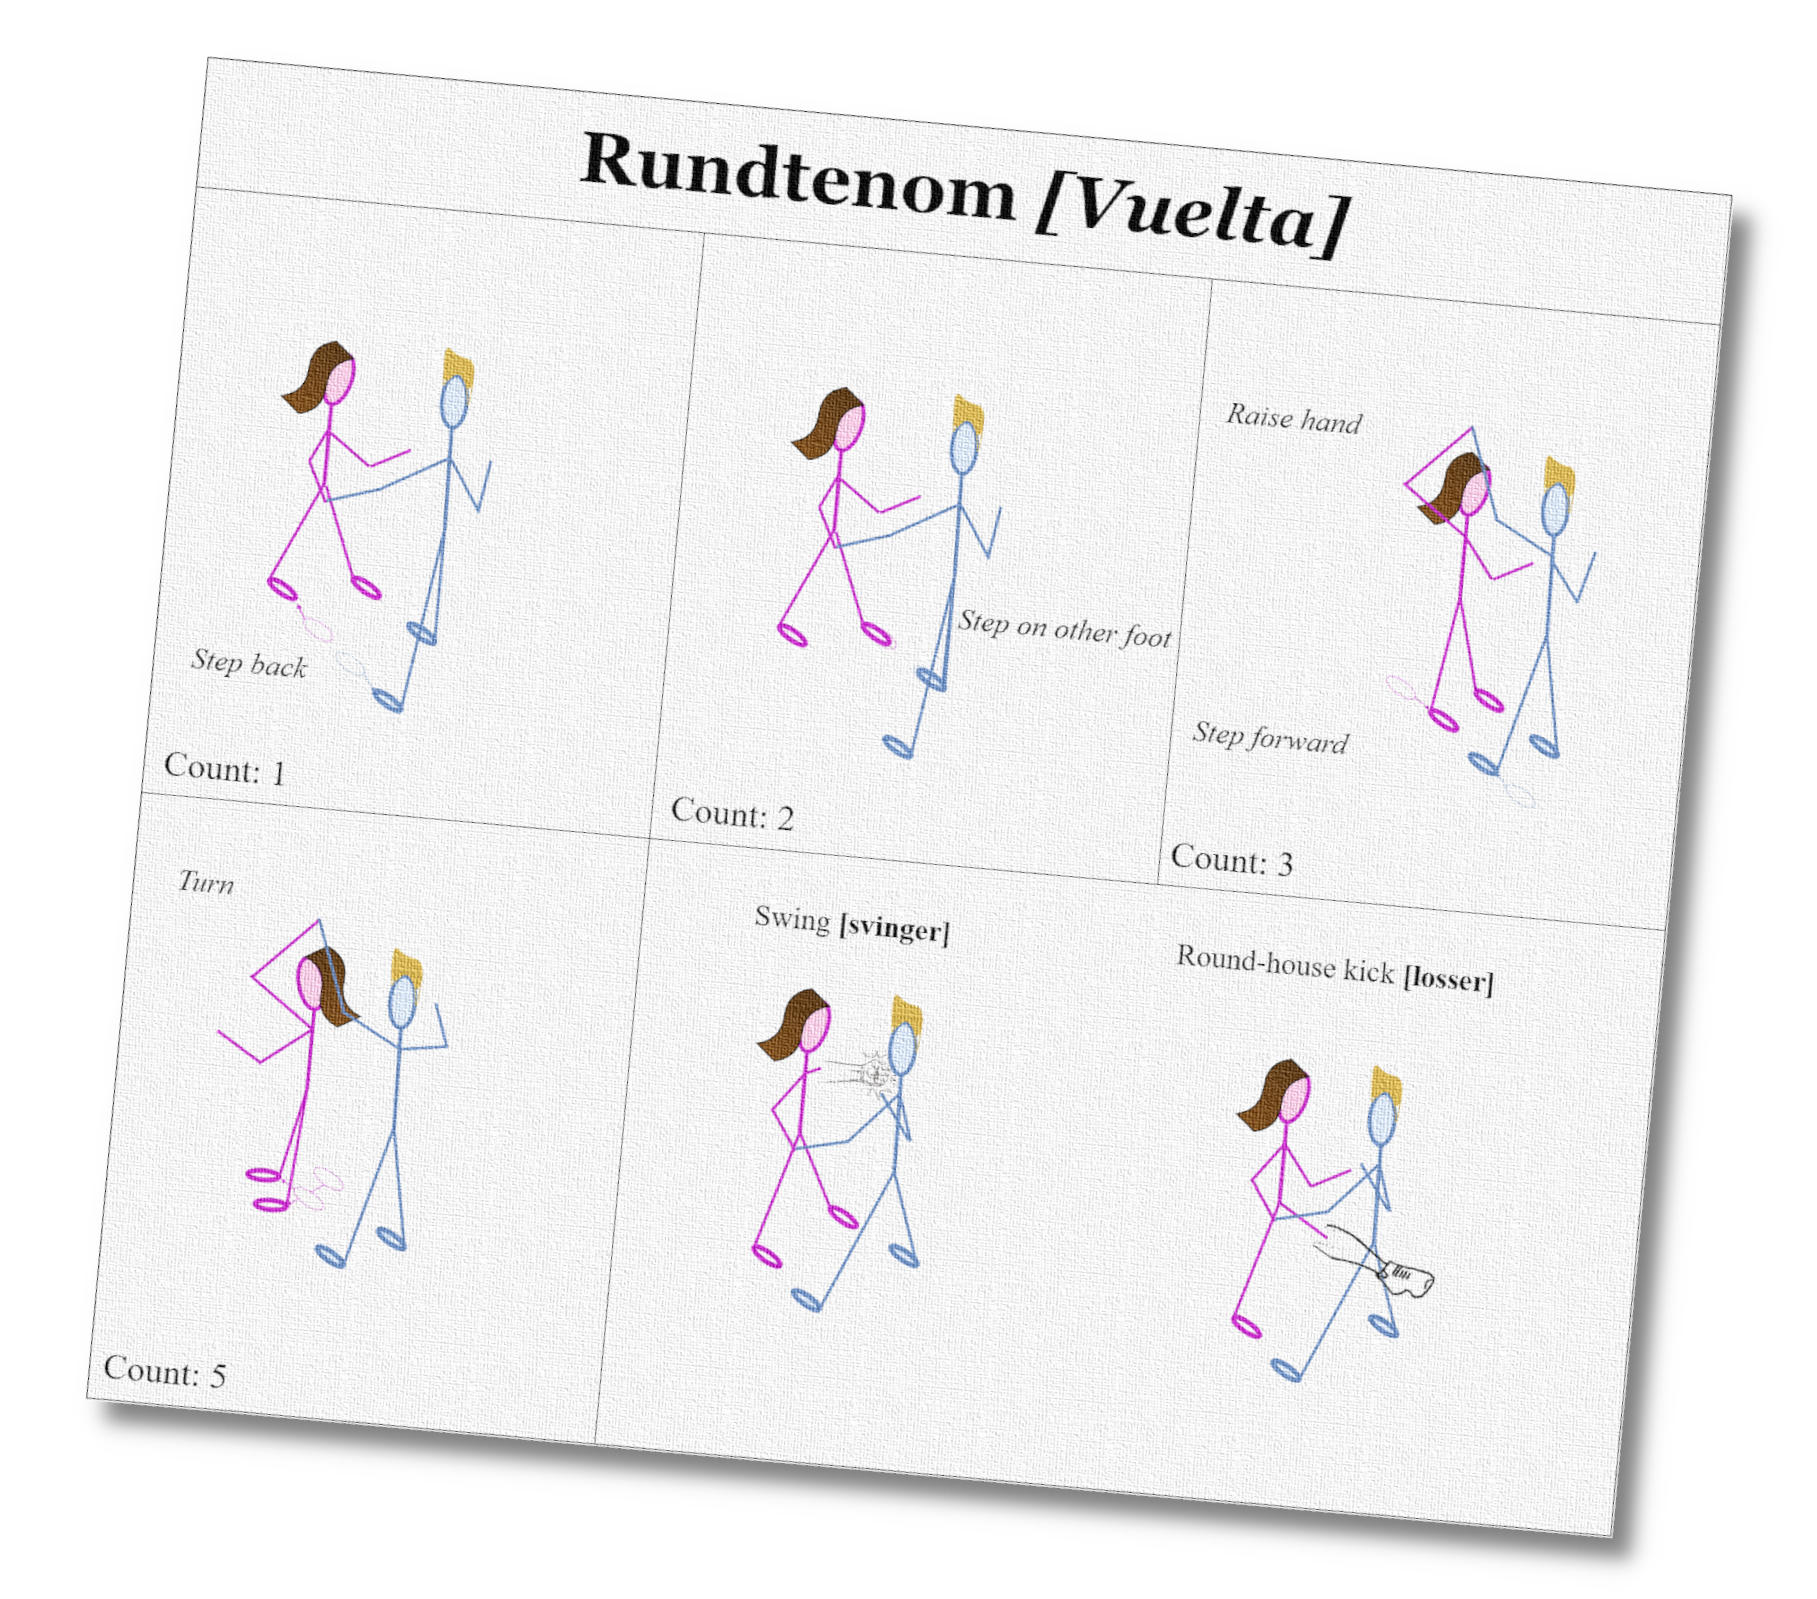
\includegraphics[scale=0.15]{02-Description/diagram-vuelta-present}
\end{center}
\subparagraph*{Description}
As both the Cuban Salsa and the \sovs name for this figure suggests, this move is all about spinning. For \gal at least.\\
The move starts out as \sovsguapea, with both parties stepping back on the $1^{st}$ count, and stepping back to the starting position on the $3^{rd}$ count, but in the \sovsvuelta \dude will raise his left hand on the $3^{rd}$ count to let \gal know that she is about to do some spinning. On count 5, \gal will step forward with her \textbf{left} foot, and proceed to do an outside turn (around her right shoulder)  on counts 6 and 7. 
\subparagraph*{Suggestions for attacking}
Given that the move finishes off with a spinning motion on the part of \gal, any type of attack that can utilize the energy of the spinning motion to generate force will work really well, like for instance:

\begin{itemize}
  \item \attsvinger 
  \item \attack{lav svinger} 
  \item \attlosser
  \item \atthestehilsen
\end{itemize}

\pagebreak{}
\section*{\Sovsenchufla [\Salsaenchufla]}
\begin{center}
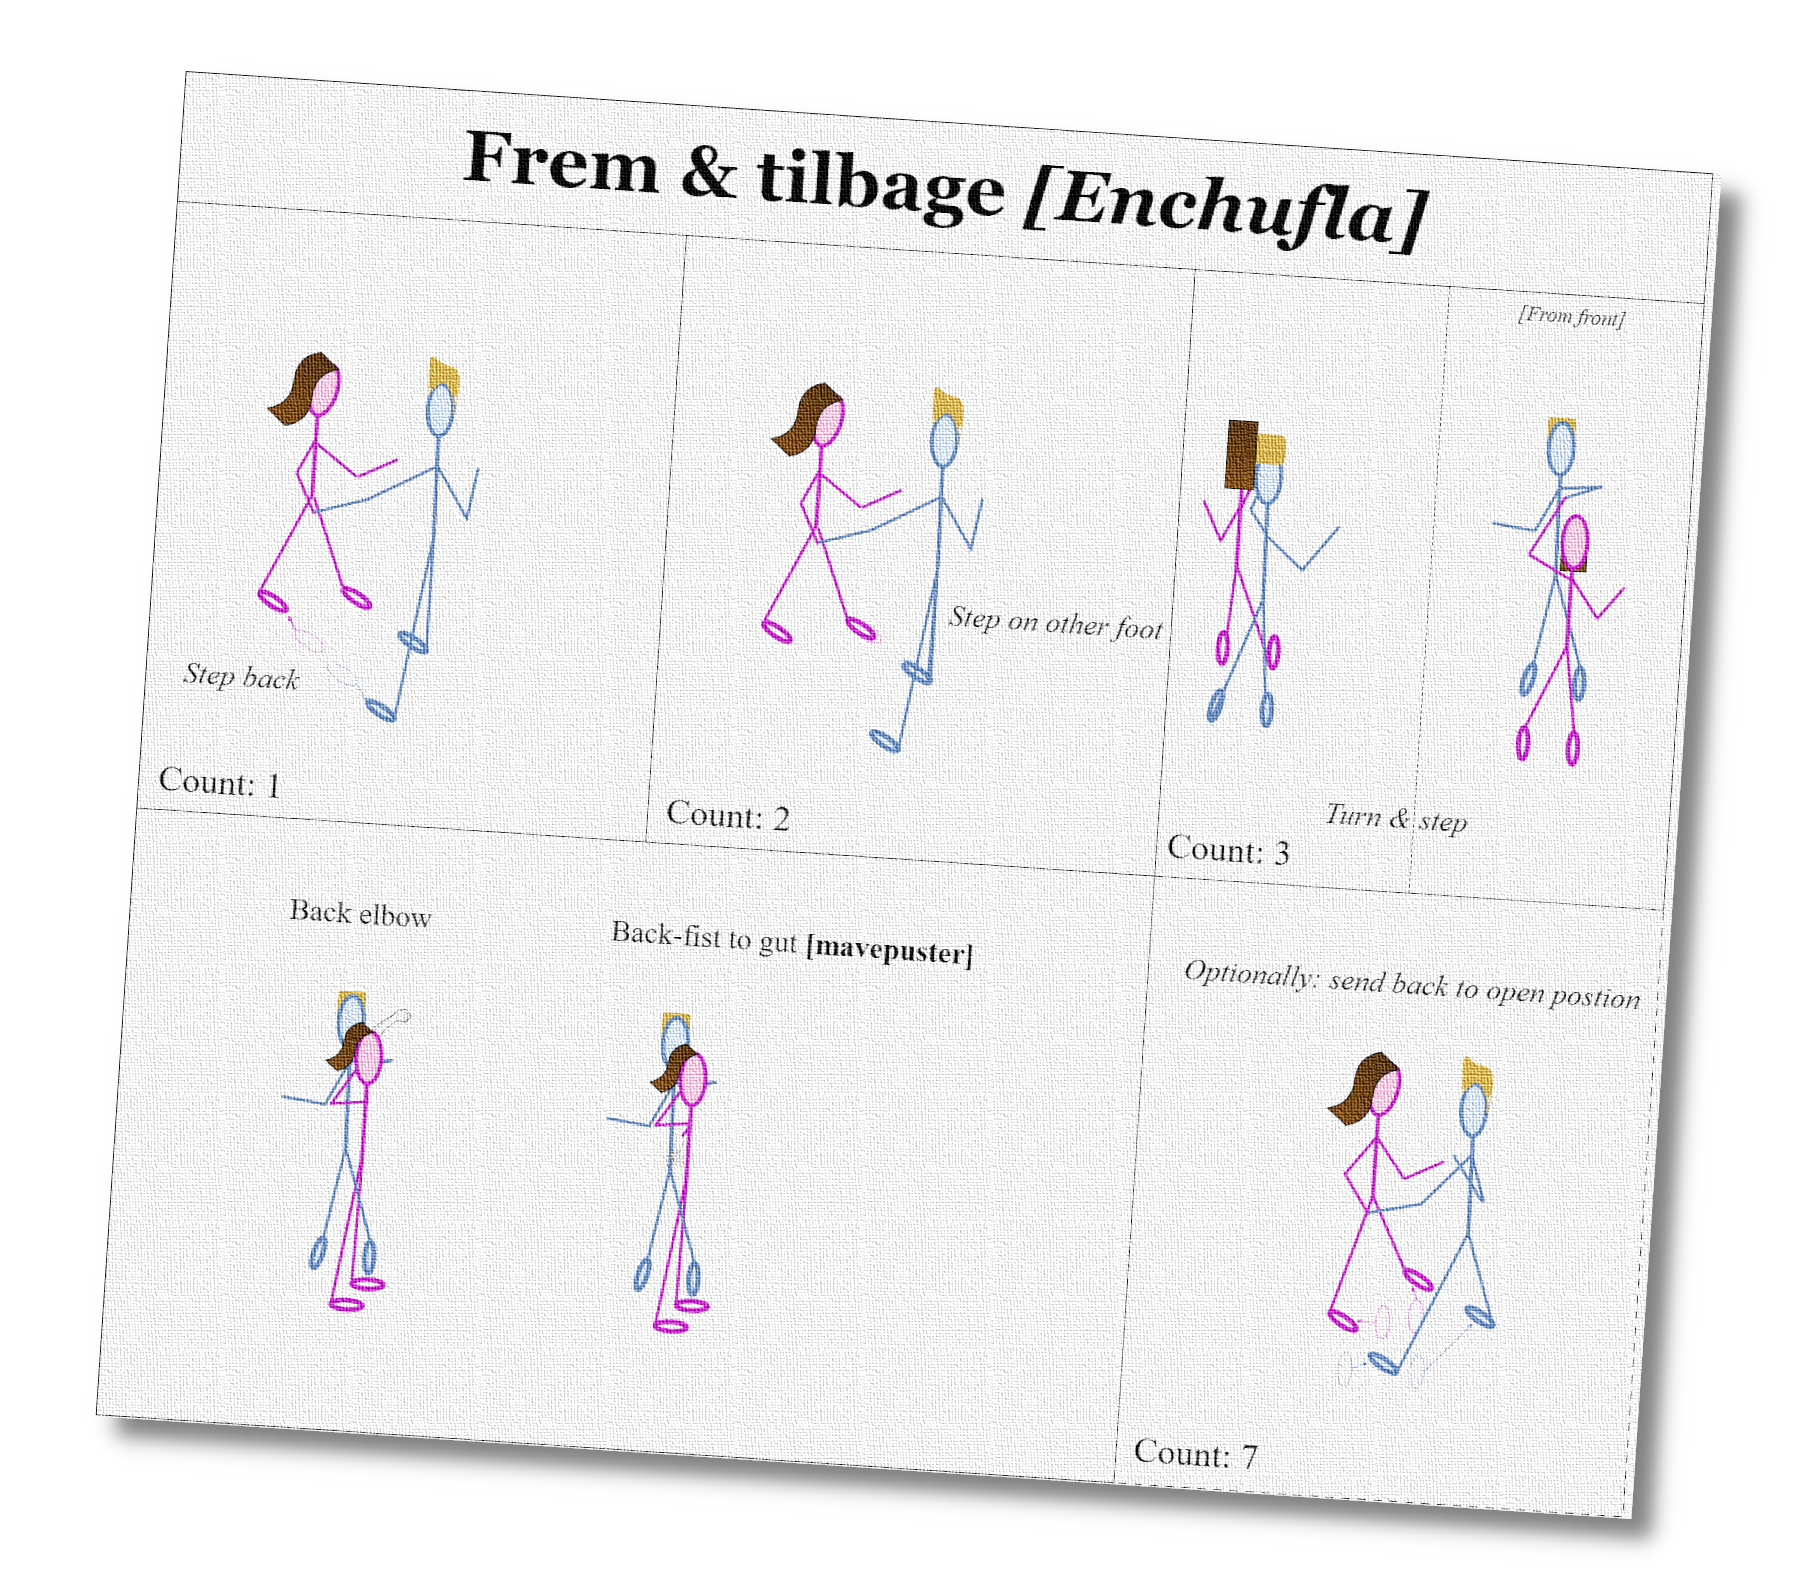
\includegraphics[scale=0.15]{02-Description/diagram-enchufla-present}
\end{center}

\subparagraph*{Description}
\Sovsenchufla is another move for \dude and \gal to exchange places during 8 counts, and is often used in Cuban Salsa as part of other figures. On the $1^{st}$ count, both \dude and \gal will step back as in \sovsguapea, but unlike in \sovsguapea, they will both travel forwards on the $2^{nd}$ and $3^{rd}$ counts. Additionally, on the $2^{nd}$ count, \dude will bring his \textbf{left} hand (which is holding on to \gal's \textbf{right} hand throughout the move) up and infront of their centers, inviting \gal to cross infront of him, with her back to him. At the end of the $3^{rd}$ count, both parties turn towards each other. Counts 5, 6 and 7 proceed as for \sovsguapea. 
\subparagraph*{Suggestions for attacking}
This is one of those moves that really allows \gal to rid herself of a drunken or unattentive partner! If she starts her spinning motion as she crosses infront of \dude, and hits him with a \attkaffekage (back elbow) (thereby completing the Danish saying: \textit{``Kaffe \& kage, frem \& tilbage''} to the face, she will send an unambigous message to \dude, that he should look for another place to spend the night. Of course, it may be the case that \dude is not as drunk/unattentive as he looks, and is able to catch the elbow in-flight, and in this case, he has little choice but to push her back in what is known in \sovs as \sovsenchufla$^{2}$ [\figsalsa{enchufla doble}]. \\
\gal also has the option to postpone her spinning motion and attack until the $3^{rd}$ count, but will likely have to throw an attack with a longer reach at \dude, like for instance a \attbagknytter or \attsideaxe.


\pagebreak{}
\section*{\Sovsvacilala [\Salsavacilala]}
\begin{center}
\includegraphics[scale=0.15]{02-Description/diagram-vacílala-present}
\end{center}
\subparagraph*{Description }
\Sovsvacilala is initiated already on the preceeding move (typically \sovsguapea), as \dude let's \gal know that \textit{``something is up'}', by pushing a little harder than usual with his free hand in order to open up their position. As such, \sovsvacilala starts with the both of them looking in the same direction.
On the first count, \dude gently motions \gal's right hand in a spinning motion inwards as he steps to move past her on the outside. \gal performs a single (or double/tripple) spin moving past and away from \dude. 
On the 5-count \dude steps toward \gal, in order to close the distance and prepare for \sovsdile.

\subparagraph*{Suggestions for attacking}
Given the rather large distance between the 2 on count 4 and 5, and the fact that \gal is free from contact with \dude and hence enjoys full freedom of motion, it is a great time for her to show off her athletic abilities and hit him with some long-distance kicking. \gal can opt for a \atttrykker directed towards \dude's torso, or she could adjust her body sideways and go for a \attsidetrykker. She can go for the power-up and preface the \attsidetrykker with stepping into the kick with her rear leg, which is sure to send \dude flying if he is not attentive which will most certainly aid \gal in establishing dominance on the dance floor.\\
If \gal feels like showing off, she can pull out the old kick-combo classic, the \attfootjuglar faking a round-house kick and following up with a \atthestehilsen from the opposite foot.  
